\chapter{Metodologia} \label{metodologia}

Neste capítulo os detalhes envolvidos na geração das imagens de CAPTCHAs são expostos. Em seguida, definimos as grandezas de interesse que nos permitem acessar a qualidade dos modelos treinados. Por fim, as etapas de treino e validação são formalizadas.


\section{Geração dos CAPTCHAs}

Todos os exemplos foram gerados utilizando a biblioteca SimpleCaptcha\cite{simplecaptcha}. Ao total, foram gerados $30000$ pares imagem-token, diferentes cores e efeitos e tokens sob o alfabeto (ordenado) $\Sigma = \{0123456789abcdefghijklmnopqrstuvwxyz\}$ com comprimento fixo em 5. Dentre os efeitos escolhidos, enfatizamos que variações nas cores de fundo, desenho de grades, adição de linhas aleatórias e deformação em explosão são técnicas efetivas para construir desafios fáceis para humanos e difíceis para computadores de acordo com estudo conduzido por \cite{lectures2005HIP}. Uma pequena amostra das imagen-token geradas pode ser vista na Fig.\ref{imgcaptchas}. 


Considere $D = {(x, y)}$ o conjunto formado por todos os pares de imagem-token gerados. Cada exemplo é formado por um tensor imagem $x$ e uma matriz $y$ representando o token, de dimensões $(200, 50, 3)$ e $(5, 36)$, respectivamente. Cada entrada $x_{ijk} \in \Re[0,1]$ representa a intensidade do pixel localizado na posição $(i,j)$ e canal $k$. A entrada $y_{ij} \in \Re[0,1]$ foi codificada utilizando-se a técnica \textit{one-hot encoding}, onde $i$ representa a posição na sequência $w$ e $j$ o índice no vocabulário do caractere nessa posição, de modo que 
\begin{equation}
   y_{ij}= 
	\begin{cases}
		1,	& \text{se } w_i = \Sigma_j\\
		0,  & \text{caso contrário.}
	\end{cases}
\end{equation}
Essa codificação nos permite interpretar $y$ como sendo uma distribuição de probabilidade. Seja $ord(w_i)$ o índice no vocabulário tal que $w_i = \Sigma_{ord(w_i)}$ e $c$ o caractere em $w_i$, temos que $y_{ij = ord(c)} = p(w_i=c|x) = 1$ e $y_{i\;j \neq ord(c)} = p(w_i \neq c|x) = 0$, isto é, temos $100\%$ de certeza de que o caractere em $w_i$ é $c$.

$D$ foi reordenando de forma aleatória e separado em dois subconjuntos:
o conjunto de treino, $D_{tr}$, com $\frac{2}{3}$ do total de pares, e o conjunto de validação, $D_{val}$, com os demais exemplos. Devido a natureza combinatória do espaço de imagens possíveis ($36^5$ tokens $\times$ $255^3$ cores de fundo $\times$ espaço de todas as pertubações possíveis), acreditamos que não existam exemplos em comum nesses dois conjuntos. 

\begin{figure}[ht]
	\begin{subfigure}{.5\textwidth}
		\centering
	 	
\includegraphics[width=.9\linewidth]{figuras/7103_b26bf.png}
		\caption{b26bf}
	\end{subfigure}
	\begin{subfigure}{.5\textwidth}
		\centering
		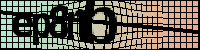
\includegraphics[width=.9\linewidth]{figuras/9456_ep8nb.png}
		\caption{ep8nb}
	\end{subfigure}%
	\vspace{.05\linewidth}

	\begin{subfigure}{.5\textwidth}
		\centering
		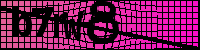
\includegraphics[width=.9\linewidth]{figuras/21856_b7rw8.png}
		\caption{b7rw8}
	\end{subfigure}
	\begin{subfigure}{.5\textwidth}
		\centering
		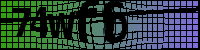
\includegraphics[width=.9\linewidth]{figuras/19816_74wf6.png}
		\caption{74wf6}
	\end{subfigure}%
	\vspace{.05\linewidth}

	\begin{subfigure}{.5\textwidth}
		\centering
		
\includegraphics[width=.9\linewidth]{figuras/12248_dnyny.png}
		\caption{dnyny}
	\end{subfigure}
	\begin{subfigure}{.5\textwidth}
		\centering
		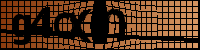
\includegraphics[width=.9\linewidth]{figuras/8873_g4cxh.png}
		\caption{g4cxh}
	\end{subfigure}%
	\vspace{.05\linewidth}
	\caption{Exemplos de CAPTCHAs gerados e seus respectivos tokens.}
	\label{imgcaptchas}
\end{figure}


\section{Treino e Validação}

Em todos os experimentos as redes foram inicializadas segundo a heurística proposta em \cite{HeZR015relu}. Após a inicialização, seguem-se repetidas épocas de aprendizado até que o critério de parada (descrito mais adiante) seja satisfeito ou um máximo de $T^{max}$ épocas seja atingido.

Uma época de aprendizado consiste em duas etapas: treino e validação. Durante o treino, um subconjunto $D_{batch} \subset D_{tr}$ é sorteado ao acaso. Os parâmetros da rede são atualizados utilizando o algoritmo Adam\cite{adam_op} com taxa de aprendizado $l_r$ de forma a minimizar o erro nesse subconjunto. A etapa de treino se encerra após $|D_{tr}|/|D_{batch}|$ atualizações. Na etapa de validação, as grandezas de interesse são calculadas para $D_{tr}$ e $D_{val}$ e salvas para posterior análise.

Para selecionar o valor do hiper-parâmetro $l_r$, foram realizados experimentos usando diferentes valores de $l_r$ e $T^{max}=10$ épocas para cada arquitetura. A partir dos experimentos, selecionamos manualmente os limites inferior e superior, ($l_r^-$, $l_r^+$), que apresentam o melhor compromisso entre velocidade de aprendizado e estabilidade. O experimento é então executado novamente utilizando decaimento linear para $l_r$ de acordo com a equação:
\begin{equation}
l_r(t) = l_r^+ + (l_r^- - l_r^+) * \frac{t}{T_{max}-1},
\end{equation}
onde $t = 0, 1, 2, \ldots, T_{max}-1$, onde $t$ é a época atual.

O critério de parada é definido por uma heurística semelhante às definidas por \cite{lutz_early_stop}. O aprendizado leva no mínimo 10 e no máximo 50 épocas. Após a etapa de validação o aprendizado é interrompido prematuramente se um dos dois critérios forem verificados: o erro calculado em $D_{val}$ na época atual ultrapasse em mais de $10\%$ o menor valor do erro nesse conjunto nas épocas anteriores; o valor do erro atual em $D_{tr}$ seja maior do que $97\%$ da média dos cinco últimos erros nesse conjunto. Ou seja, o treinamento é parado prematuramente se for detectado \textit{overfit} ou se não houver melhora significativa em relação aos últimos valores.

Todos os experimentos realizados nesse trabalho foram executados em um pentium core i5 com 8gb de RAM utilizando a biblioteca tensorflow. Sendo este o limite prático para o tamanho dos modelos e da base de treino. 

\section{Grandezas de interesse}

Na secção de fundamentação teórica de redes neurais (sec. \ref{sec:neurais}), vimos que cada arquitetura é parametrizada $\Theta$. Mais especificamente, cada uma das arquiteturas utilizadas neste trabalho possui como parâmetros um conjuntos de números reais. Assim, definimos a complexidade do modelo, para fins de comparação, como a soma da quantidade de parâmetros de cada camada da arquitetura. Para treinar e acessar a qualidade dos modelos, consideramos as grandezas definidas à seguir. Para todas as definições, considere $D$ um conjunto de exemplos, $(x,y) \in D$ e $\hat{y} = f^{\Theta}(x)$ a distribuição de probabilidade inferida, como descrito anteriormente. 

A entropia cruzada pode ser interpretada como uma medida de divergência entre duas distribuições de probabilidade. O erro associado ao inferir $\hat{y}$ quando a verdadeira distribuição deveria ser $y$, por caractere, é dado por
\begin{align}
	H_i(y, \hat{y}) &= -\sum_j y_{ij} \log_2{\hat{y}_{ij}} \\
					&= -\log_2{\hat{y}_{i\;ord(wi)}}
\end{align}
onde utilizamos o fato de $y_{ij} = 0$ exceto em $j = ord(w_i)$. Em outras palavras, a entropia associada ao classificador da posição $i$ é o logaritmo da probabilidade predita para o caractere correto nessa posição. Definimos o erro esperado do classificador $i$ no subconjunto $D$  
\begin{equation} \label{lossi} 
	J_i^{(D)} = \frac{1}{|D|} \sum_{(x,y) \in D} H_i(y, \hat{y}).
\end{equation}
e erro total de predição do token com a soma dos erros em cada posição:
\begin{equation} \label{loss}
	J^{(D)} = \sum_{i} J_i^{(D)}
\end{equation}
Durante o treino tentaremos minimizar a \ref{lossi} para cada classificador, e o erro total do modelo é estimado pela equação \ref{loss}.

Uma estimativa da probabilidade de acerto por caractere é dada pela acurácia de cada classificador, isto é, o número de acertos do caractere $i$ no conjunto $D$, $N_i$, normalizado pelo tamanho do conjunto $D$: 
\begin{equation}
	\hat{p}_i^{(D)} = acc_i^{(D)} = \frac{N_i}{|D|}
\end{equation}
Supondo que os $\hat{p}_i^{(D)}$ sejam independentes entre si, podemos definir uma estimativa para a probabilidade de acerto do token como o produto das probabilidades individuais:
\begin{equation} \label{eq:phat}
	\hat{p_w}^{(D)} = \prod_{i} \hat{p}_i^{(D)}.
\end{equation}
Adicionalmente, definimos a acurácia do modelo como sendo o número de acertos na predição do token, $N_w$, normalizado pelo tamanho do conjunto:
\begin{equation} \label{eq:accw}
	acc_w^{(D)} = \frac{N_w}{|D|}.
\end{equation}
Chamamos a atenção de que as equações \ref{eq:phat} e \ref{eq:accw} não necessariamente representam a mesma grandeza, fornecendo duas estimativas diferentes para a qualidade do modelo.

Quanto ao tempo dos algoritmos, estamos interessados em duas medidas: o tempo de treino por época, $\tilde{\tau}$, o tempo total (treino e validação) por época, $\tau$, e o tempo até convergência $T$.